Haizea supports a variety of resource leases. There's a more detailed description of what a lease is in the What is Haizea? page, and this page just describes the supported types of leases. Throughout this page, let's assume you have a 4-node cluster, and that you want to lease parts of that cluster over time. We'll represent the four nodes over time like this:

\section{"Advance Reservation" lease}

An advance reservation, or AR, lease is a lease that must begin and end at very specific times. For example, the following lease starts at 1pm and ends at 2pm:

\begin{center}
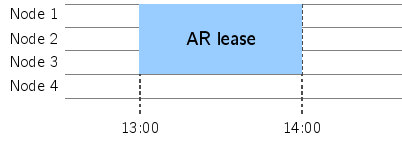
\includegraphics{images/lease_ar.png}
\end{center}

Haizea can schedule this type of lease, which is particularly useful when you need resources at a specific time (for example, to coincide with a lecture, an experiment, etc.)

\section{Preemptible best-effort lease}

Sometimes, you know you need resources, but you don't need them at a specific time. In fact, you're perfectly content to wait until there are enough resources available for your lease:

\begin{center}
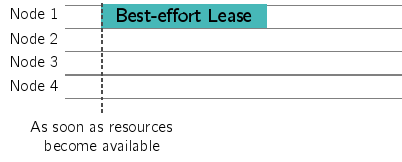
\includegraphics{images/lease_be1.png}
\end{center}


When you request a best-effort lease, your request gets placed in a queue, which is processed in a first-come-first-serve basis (the queue uses backfilling algorithms to improve resource management). The downside of this type of lease, of course, is that you may have to wait a while until resources are allocated to your lease:

\begin{center}
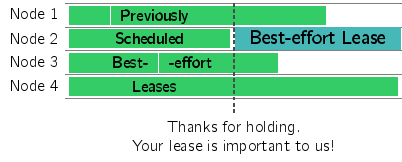
\includegraphics{images/lease_be2.png}
\end{center}

Furthermore, your lease may be running a program unattended which can be safely paused for a while (since no one is interactively using the lease resources). By requesting a preemptible lease, you allow your resources to be preempted by higher-priority leases, like advance reservations:

\begin{center}
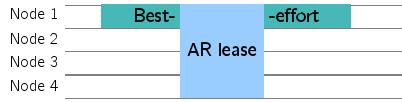
\includegraphics{images/lease_be3.png}
\end{center}

Preemptible best-effort leases are good for running batch jobs, or any non-interactive work. The Haizea paper Combining Batch Execution and Leasing Using Virtual Machines showed how using the suspend/resume capability of virtual machines allowed AR and best-effort leases to be scheduled together efficiently, overcoming the utilization problems typically associated with ARs.

\section{Non-preemptible best-effort lease}

But what if you're willing to wait for your resources to become available, but don't want them to be preempted? (e.g., if you want to use them interactively). Well, it's as simple as requesting a non-preemptible best-effort lease. Once your request makes it through the queue, and your lease is allocated resources, no one is taking them away.

\section{Immediate lease}

In some cases, you may need resources now. As in \emph{right now}:

\begin{center}
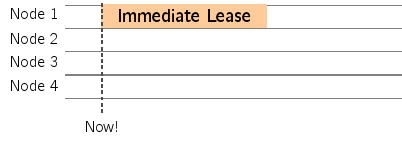
\includegraphics{images/lease_im.png}
\end{center}


Furthermore, if you can't get them right now, you're just not interested in anything else the resource provider has to offer. You're not going to request resources in the future, and you're certainly not going to be put on a queue. This is essentially the type of lease that many cloud systems offer (although the definition of "right now" varies wildly). Take into account that an immediate lease may still take a while to setup (VM image deployment, etc.). This type of lease in Haizea may evolve in the future into an "urgent lease", where "right now" really does mean "right now".

\section{Coming soon}

The following types of leases are coming soon to a lease manager near you:

\subsection{Best-effort with deadlines}

In some cases, when you say "best effort", you really mean "best effort, but be reasonable". Sure, you're willing to wait for your resources, but you may need them before a deadline.

\begin{center}
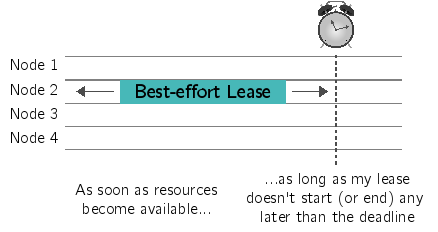
\includegraphics{images/lease_deadline.png}
\end{center}


For example, let's say you want a 16-node cluster sometime today to run a test program. You're not particularly picky about when you get the cluster, as long as it happens today and you're given sufficient warning of when your lease will be available. In the future, you will be able to tell Haizea that you have a deadline, and Haizea will either get the resources to you by then, or tell you that the deadline is simply unfeasible.

\subsection{Negotiated leases}

If you've ever entered into any sort of non-computational lease agreement, you know that agreeing on the lease terms rarely involves the lessor instantly being on the same page as you. Rather, it involves a fair amount of haggling. Besides, if your computational needs are flexible, so should your lease manager (c'mon, are you sure you mean "exactly at 2pm"? maybe you meant to say "at some point this afternoon"?). In the future, you will be able to negotiate your leases with Haizea:

\begin{center}
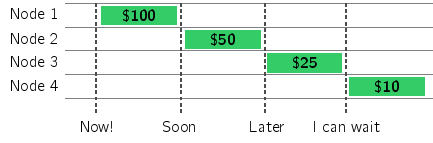
\includegraphics{images/lease_negotiate.png}
\end{center}


So, hey, maybe we can't get you that shiny AR you want at 2pm, but how about I get you twice the resources at an off-peak time? I'll even throw in a discount. And free air conditioning.